\section{Improved Mean Flows}

\begin{figure}[t]
    \centering
    \vspace{-1em}
    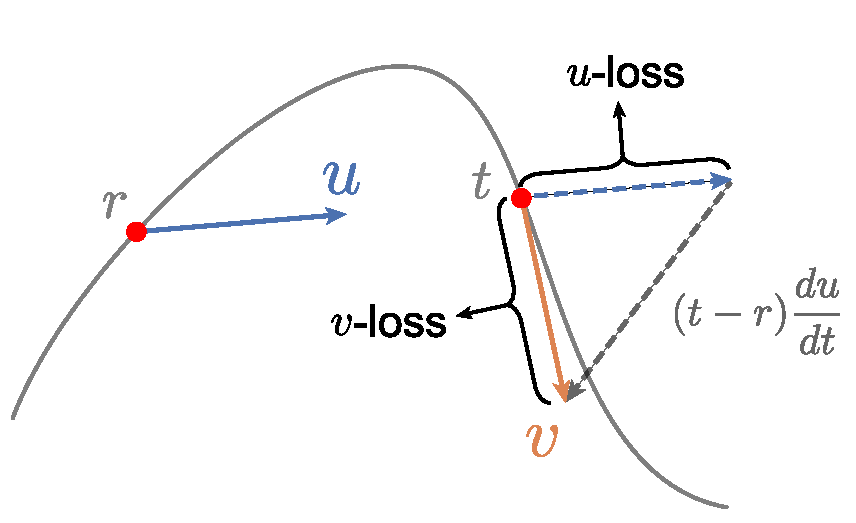
\includegraphics[width=0.75\columnwidth]{figs/demo.pdf}
    \caption{\textbf{MeanFlow as $v$-loss.}
    Original MeanFlow (MF)~\cite{mf} models the average velocity $u$ and train the network $u_\theta$ via a \textbf{$u$-loss} parameterized by $u_\theta$ itself. We show that MF can be reformulated as a \textbf{$v$-loss} re-parameterized by $u_\theta$, driven by the MeanFlow identity in \cref{eq:mf-identity2}.
    }
    \label{fig:imf-mf-teaser} 
\end{figure}

We identify and address two challenges of the original MF model. \textbf{(i)} The apparent target in \cref{eq:u-tgt} depends on the network. We aim for a more standard regression formulation (\cref{sec:v-pred}). \textbf{(ii)} To extend the MeanFlow identity for supporting CFG, original MF fixes the guidance scale before training. We relax this constraint and allow for flexible CFG (\cref{sec:method-cfg}). We then introduce an improved architecture for handling many types of conditions by in-context conditioning (\cref{sec:method-arch}).



\subsection{MeanFlow as \texorpdfstring{$v$-loss}{v-loss}}
\label{sec:v-pred}

\cref{eq:mf-loss} suggests that original MF~\cite{mf} is a \textbf{$u$-loss} parameterized by \textbf{$u$-pred}. In this subsection, we first show that the original MF can be reformulated as a \textbf{$v$-loss} (\ie instantaneous velocity) \textit{re-parameterized} by \textbf{$u$-pred}. This gives us a network-independent target. See \cref{fig:imf-mf-teaser}.

This reformulation reveals a hidden issue: the prediction function for $v$ requires access to \textit{unknown} quantities, not just $z_t$. We provide a solution to remedy this issue. With our reformulation, we arrive at a more standard regression problem. 

\paragraph{Reformulating MeanFlow as $v$-loss.}
While MF aims to compute $u$-loss, the true target $u$ is not accessible. As a result, the target $\utgt$ has a term approximated by $\mathtt{JVP}(u_\theta; e-x)$ in \cref{eq:u-tgt}, which is not a standard regression target. 
We notice that the \textit{instantaneous} velocity $v$ can serve as a more feasible target. We can rewrite the MeanFlow identity (\ref{eq:mf-identity}) as (see also \cref{fig:imf-mf-teaser}):
\begin{equation}
v(z_t) \;=\; u(z_t)\;+\;(t-r)\,\frac{d}{dt}\,u(z_t).
\label{eq:mf-identity2}
\end{equation}
Here, $v$ on the left-hand side can serve as a target, as in standard Flow Matching; the \textit{compound function} on the right-hand side can be parameterized by $u_\theta$. We denote the \mbox{(re-)parameterized} compound function as $V_\theta$:
\begin{equation}
    V_\theta
    \triangleq u_\theta\,(z_t) + (t-r)\,\sgjvp(u_\theta; e-x),
\label{eq:big-V}
\end{equation}
where $\sgjvp$ denotes stop-gradient on the $\ddt u_\theta$ outcome (we will discuss stop-gradient later).
Then we obtain a Flow Matching-like objective function, similar to \cref{eq:fm-loss}:
\begin{equation}
    \label{eq:V-loss}
    \mathbb{E}_{t,r,x,e}\|V_\theta - (e-x)\|^2.
\end{equation}
It is easy to show that the reformulation in (\ref{eq:big-V})(\ref{eq:V-loss}) is fully \textit{equivalent} to the original MF objective in (\ref{eq:u-tgt})(\ref{eq:mf-loss}).
This suggests that \textit{MeanFlow can be viewed as $v$-loss re-parameterized by $u_\theta$}. Such re-parameterization in \cref{eq:big-V} is driven by the MeanFlow identity in \cref{eq:mf-identity2}.

This reformulation reveals a new issue: $V_\theta$ in \cref{eq:big-V} does not only take $z_t$ as input, but more importantly, also takes $e - x$ as another input. Formally, our parameterized compound function $V_\theta$ is:
\begin{equation}
V_\theta(z_t, e - x).
\end{equation}
This is illustrated in \cref{fig:teaser}\textbf{(a)}.
From the perspective of a standard regression formulation (\eg \cref{eq:fm-loss}), this is not a fully legitimate prediction function. We will show the negative effect of this extra input in \cref{fig:loss}. 

\definecolor{codeblue}{rgb}{0.25,0.5,0.5}
\definecolor{codesign}{RGB}{0, 0, 255}
\definecolor{codefunc}{rgb}{0.85, 0.18, 0.50}


\lstdefinelanguage{PythonFuncColor}{
  language=Python,
  keywordstyle=\color{blue}\bfseries,
  commentstyle=\color{codeblue},
  stringstyle=\color{orange},
  showstringspaces=false,
  basicstyle=\ttfamily\small,
  literate=
    {+}{{\color{codesign}+ }}{1}
    {-}{{\color{codesign}- }}{1}
    {*}{{\color{codesign}* }}{1}
    {/}{{\color{codesign}/ }}{1}
    {sample_t_r}{{\color{codefunc}sample\_t\_r}}{1}
    {randn_like}{{\color{codefunc}randn\_like}}{1}
    {jvp}{{\color{codefunc}jvp}}{1}
    {stopgrad}{{\color{codefunc}stopgrad}}{1}
    {metric}{{\color{codefunc}metric}}{1}
}

\lstset{
  language=PythonFuncColor,
  backgroundcolor=\color{white},
  basicstyle=\fontsize{9pt}{9.9pt}\ttfamily\selectfont,
  columns=fullflexible,
  breaklines=true,
  captionpos=b,
}

\newcommand{\safeColorbox}[2]{%
  \begingroup
  \setlength{\fboxsep}{0pt}%
  \colorbox{#1}{\strut #2}%
  \endgroup
}

\begin{algorithm}[t]
\centering
\caption{{improved MeanFlow}: training.\\
{\scriptsize Note: in PyTorch and JAX, \texttt{jvp} returns the function output and JVP.}}
\label{alg:code}
\begin{minipage}{0.98\linewidth}
\begin{lstlisting}[language=PythonFuncColor, escapechar=`]
# fn(z, r, t): function to predict u
# x: training batch

t, r = sample_t_r()
e = randn_like(x)

z  = (1 - t) * x + t * e

# instantaneous velocity v at time t
v = fn(z, t, t)

# predict u and dudt
u, dudt = jvp(fn, (z, r, t), (v, 0, 1))

# compound function V
V = u + (t - r) * stopgrad(dudt)
error = V - (e - x)

loss = metric(error)
\end{lstlisting}
\end{minipage}
\end{algorithm}

\paragraph{Improved MeanFlow Parameterization.}
The reason for $V_\theta$'s dependence on $e-x$ is on $\mathtt{JVP}$, which can be traced back to the approximation in \cref{eq:u-tgt}: the \textit{marginal} velocity $v$ in \cref{eq:total-deriv} is replaced by the \textit{conditional} velocity $v_c=e-x$. Rather than doing this replacement, we can parameterize the marginal $v$ instead. Formally, we re-define the compound function $V_\theta$ as:
\begin{equation}
    V_\theta\,(z_t) \\
    \triangleq u_\theta\,(z_t) + (t-r)\,\sgjvp\left(u_\theta; \textcolor[RGB]{255, 64, 64}{v_\theta}\right).
\label{eq:imf-vpred}
\end{equation}
Here, inside the function of $\mathtt{JVP}$, both $u_\theta$ and $v_\theta$ are network predictions: both take $z_t$ as the sole input. As such, our $V_\theta$ takes only $z_t$ as the input, which is thus a legitimate prediction function. See \cref{fig:teaser}\textbf{(b)}.

To realize ${v_\theta}$ with minimal overhead, we can reuse all or most of the network $u_\theta$.
We propose two solutions:
\begin{itemize}[leftmargin=1em, rightmargin=0em]
    \item \textbf{Boundary condition} of $u_\theta$. By definition, we have the relation: $v(z_t, t) \equiv u(z_t, t, t)$, that is, $v$ equals $u$ at $r\rightarrow t$. As such, we can simply represent $v_\theta(z_t, t)$ by $u_\theta(z_t, t, t)$. This solution introduces no extra parameters. We empirically show that this is sufficient for addressing the issue we consider here.
    \item \textbf{Auxiliary $v$-head.} Beyond directly reusing $u_\theta(z_t, t, t)$, we can add an auxiliary head in the network of $u_\theta(z_t, r, t)$ that serves as a subnetwork $v_\theta$. This introduces extra capacity for modeling $v$. It is at the cost of extra \textit{training-time} parameters, which, however, are not used at inference-time (as only $u_\theta$ is needed). 
    More details are in appendix.
    Using this head improves the results further.
\end{itemize}

\noindent
The pseudo-code of our iMF formulation is in \cref{alg:code}, where the simpler form of $v_\theta(z_t, t) \equiv u_\theta(z_t, t, t)$ is shown.

\begin{figure}[t]
    \centering
    % \vspace{-1em}
    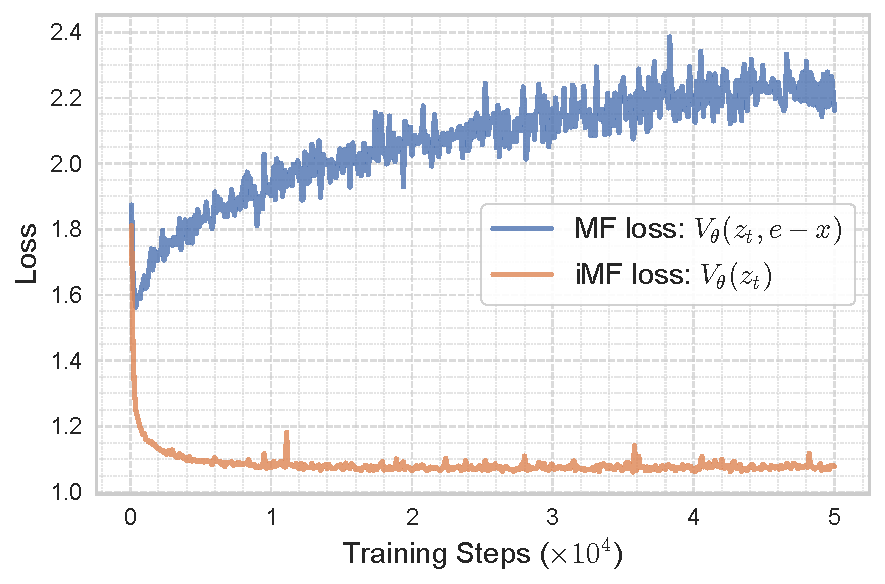
\includegraphics[width=\columnwidth]{figs/v_loss.pdf}
    \vspace{-1.5em}
    \caption{\textbf{Training losses.}
    We examine the loss of samples only with $t \neq r$, since a batch also contains samples of $t = r$, for which the $\mathtt{JVP}$ term becomes zero due to its coefficient $(t-r)$.
    Both MF and iMF can be viewed as $v$-loss, using different forms of compound $V_\theta$.
    Original MF's loss is non-decreasing and has high variance.
    (Settings: MeanFlow-B/2, trained with basic $\ell_2$ loss with no adaptive weighting, and with no CFG.)
    } 
    \vspace{-.5em}
    \label{fig:loss} 
\end{figure}

\paragraph{Comparison and Analysis.} 
In \cref{fig:loss}, we compare the training loss between the original MF and the iMF objectives (\textit{without} auxiliary $v$-head). We examine only the samples with $t \neq r$, as the $\mathtt{JVP}$ term becomes zero when $t = r$ and thus is not our focus.


Although the two formulations only differ in $V_\theta(z_t, e-x)$ and $V_\theta(z_t)$, this distinction results in strikingly different behavior. The original MF's loss has a much \textit{higher variance} and is non-decreasing\footnotemark, even though its objective can still successfully enable one-step generation.

\footnotetext{If we also include the samples of $t = r$, the original MF's overall loss can still decrease, depending on the portion of such samples.}


This comparison may look counterintuitive, because the form of $V_\theta(z_t, e-x)$ seems to ``leak'' the regression target. However, we note that the true, unique regression target for $v$-loss is not the conditional velocity $e-x$, but the marginal $v(z_t) = \mathbb{E}[\,v_c\mid z_t\,]$ in \cref{eq:marginal-v}, and therefore the leaking does not directly disclose the true $v(z_t)$. On the other hand, according to \cref{eq:total-deriv}, the input to $\mathtt{JVP}$ should not be the conditional $v_c = e-x$, but should be the marginal $v(z_t)$. 
As this is the input tangent vector to $\mathtt{JVP}$, the variance of the conditional velocity can be significantly magnified by $\mathtt{JVP}$ (\ie the Jacobian-\emph{vector} product). 
Our tangent vector is predicted by $v_\theta(z_t)$, which should have lower variance than $e - x$.
\cref{fig:loss} suggests that the large variance dominates the resulting loss.

\paragraph{About Stop-gradient.} Our formulation does not remove the stop-gradient operation, as indicated by the notation $\sgjvp$. Unlike original MF, in our case the stop-gradient is part of the prediction function $V_\theta$, not the regression target. As such, in principle, this stop-gradient is not strictly needed for the formulation itself. However, in practice, we observe that using the stop-gradient inside $V_\theta$ is still beneficial, as removing it introduces high-order gradients \wrt $\theta$ and makes optimization more difficult. 

\subsection{Flexible Guidance}
\label{sec:method-cfg}

Thus far, we have not discussed the formulation of classifier-free guidance (CFG)~\cite{cfg}. 
The original MF~\cite{mf} proposed a formulation to support 1-NFE CFG, provided that a guidance scale is \textit{fixed} at training-time.
However, a fixed guidance scale sacrifices the flexibility of adjusting this core hyperparameter at inference time. More importantly, the optimal CFG scales \textit{shift} under different settings (\cref{fig:train-inf-cfg}), and in general, a \textit{strong} model (\eg larger size, longer training, and/or more NFEs) favors a \textit{smaller} CFG scale. It is suboptimal to freeze the scale \textit{a priori}.

To address this issue, we reformulate the CFG scale as a form of \textit{conditioning}, analogous to how a model is conditioned on time steps (\eg $t$ and $r$). This enables the scale to vary at training and inference time.

\paragraph{Original MeanFlow with fixed guidance}. 
The original MF \cite{mf} considers a \textit{fixed} guidance field $v_{\text{cfg}}$: 
\begin{equation}
    \label{eq:cfg}
       v_{\text{cfg}}(z_t\mid\mathbf{c}) = \omega\,v(z_t\mid\mathbf{c}) + (1-\omega)\,v(z_t),
\end{equation}
where $\mathbf{c}$ is the class-condition, and $\omega$ is a fixed guidance scale.
Combining this definition and the MeanFlow identity, the original MF learns a \textit{class-conditional} average velocity, namely, $u_{\theta}(z_t\mid\mathbf{c})$. We omit the derivations here and refer readers to~\cite{mf}; but analogous to our reformulation in \cref{sec:v-pred}, conceptually, we can re-parameterize $u_{\theta}(z_t\mid\mathbf{c})$ into a compound function: 

\begin{equation}
    V_{\theta}(\cdot \mid \mathbf{c})
    \triangleq u_{\theta}(z_t\mid\mathbf{c}) + (t-r)\,\sgjvp.
    \label{eq:bigV-cfg}
\end{equation}
Here, for brevity, we omit the input to $V_{\theta}$ (and to $\mathtt{JVP}$), which is not our focus in this subsection: our discussion here can support both objectives in \cref{eq:big-V} (original MF) and \cref{eq:imf-vpred} (iMF).
This $V_{\theta}$ is trained to fit a target determined by a fixed $\omega$ in the original MF \cite{mf}.

\begin{figure}[t]
\centering
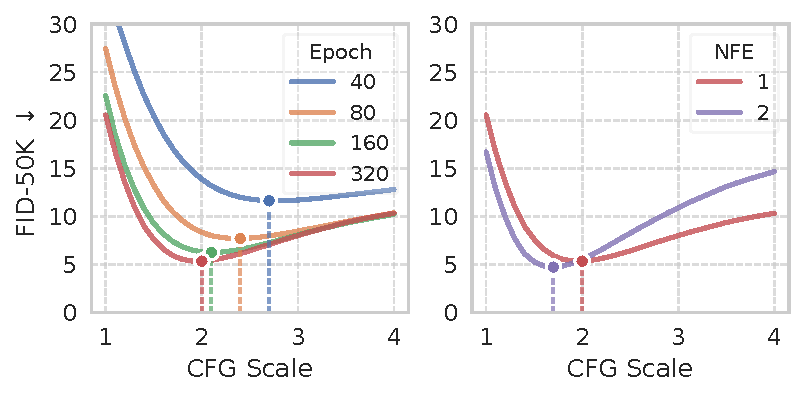
\includegraphics[width=\linewidth]{figs/train_infer_cfg.pdf}
\vspace{-1.5em}
\caption{
\textbf{Optimal CFG scales shift under different settings}.
In general, a \textit{stronger} setting has a \textit{smaller} optimal CFG scale, as reflected by increased training epochs (left) and inference steps (right).
This investigation is enabled by our flexible CFG-conditioning, where a single model can support varying CFG scales even in the single/few-NFE case. (Settings: iMF-B/2 on ImageNet 256$\times$256.)
}
\label{fig:train-inf-cfg}
\end{figure}

\paragraph{Improved MeanFlow with flexible guidance}. 
If the underlying guidance field  $v_{\text{cfg}}$ (\ref{eq:cfg}) is given by different $\omega$ values, we can still let our neural network fit each of them. To do so, we only need to allow the network to \textit{condition} on the CFG guidance scale $\omega$.
Similar strategies have been studied in multi-step methods \cite{guidancedist,nocfg,modelguidance}, which we extend to our one-step method here.

Formally, we extend \cref{eq:bigV-cfg} to:
\begin{equation}
    V_{\theta}(\cdot \mid \mathbf{c},\,\highlight{\omega})
    \triangleq u_{\theta}(z_t\mid\mathbf{c},\,\highlight{\omega}) + (t-r)\,\sgjvp,
\end{equation}
which indicates that our compound function $V_{\theta}$ can be conditioned on $\omega$, and this conditioning is handled by the network $u_{\theta}$. This is analogous to standard time-conditioning (\eg $t$ and $r$), which turns a continuous value into a learnable embedding.
At training time, the value of $\omega$ is randomly sampled from a given distribution. 
The implementation details of training with CFG conditioning is in appendix. 

\cref{fig:train-inf-cfg} shows the effect of our flexible CFG in iMF. Under different training and inference settings, the optimal guidance scale varies. Even for the \textit{same} model, training longer or using more inference steps can favor a different guidance scale, and therefore it is impossible to find the optimal scale beforehand. Our design unlocks the full potential of CFG for 1-NFE models.

\paragraph{Additional guidance conditioning.} Our formulation not only enables conditioning on a single variable $\omega$, but also allows for other guidance-related factors. We can handle CFG interval \cite{interval} under the same paradigm.

CFG interval \cite{interval} is an effective technique for improving sample diversity. In its original definition, it applies CFG only to a time interval $[t_\textrm{min}, t_\textrm{max}]$ at \textit{inference-time}. To support this behavior at training time in our one-step model, we can also view the two values $t_\textrm{min}$, $t_\textrm{max}$ as a form of conditioning. At training time, when $t$ is outside of this interval, CFG is disabled (by setting $\omega=1$).

We use the notation $\Omega=\{\omega, t_\textrm{min}, t_\textrm{max}\}$ to denote all conditions related to CFG. Each item in $\Omega$ has its own embedding. All conditions can be handled by standard adaLN-zero, or in-context conditioning, discussed next.


\begin{figure}[t]
    \centering
    \vspace{-1em}
    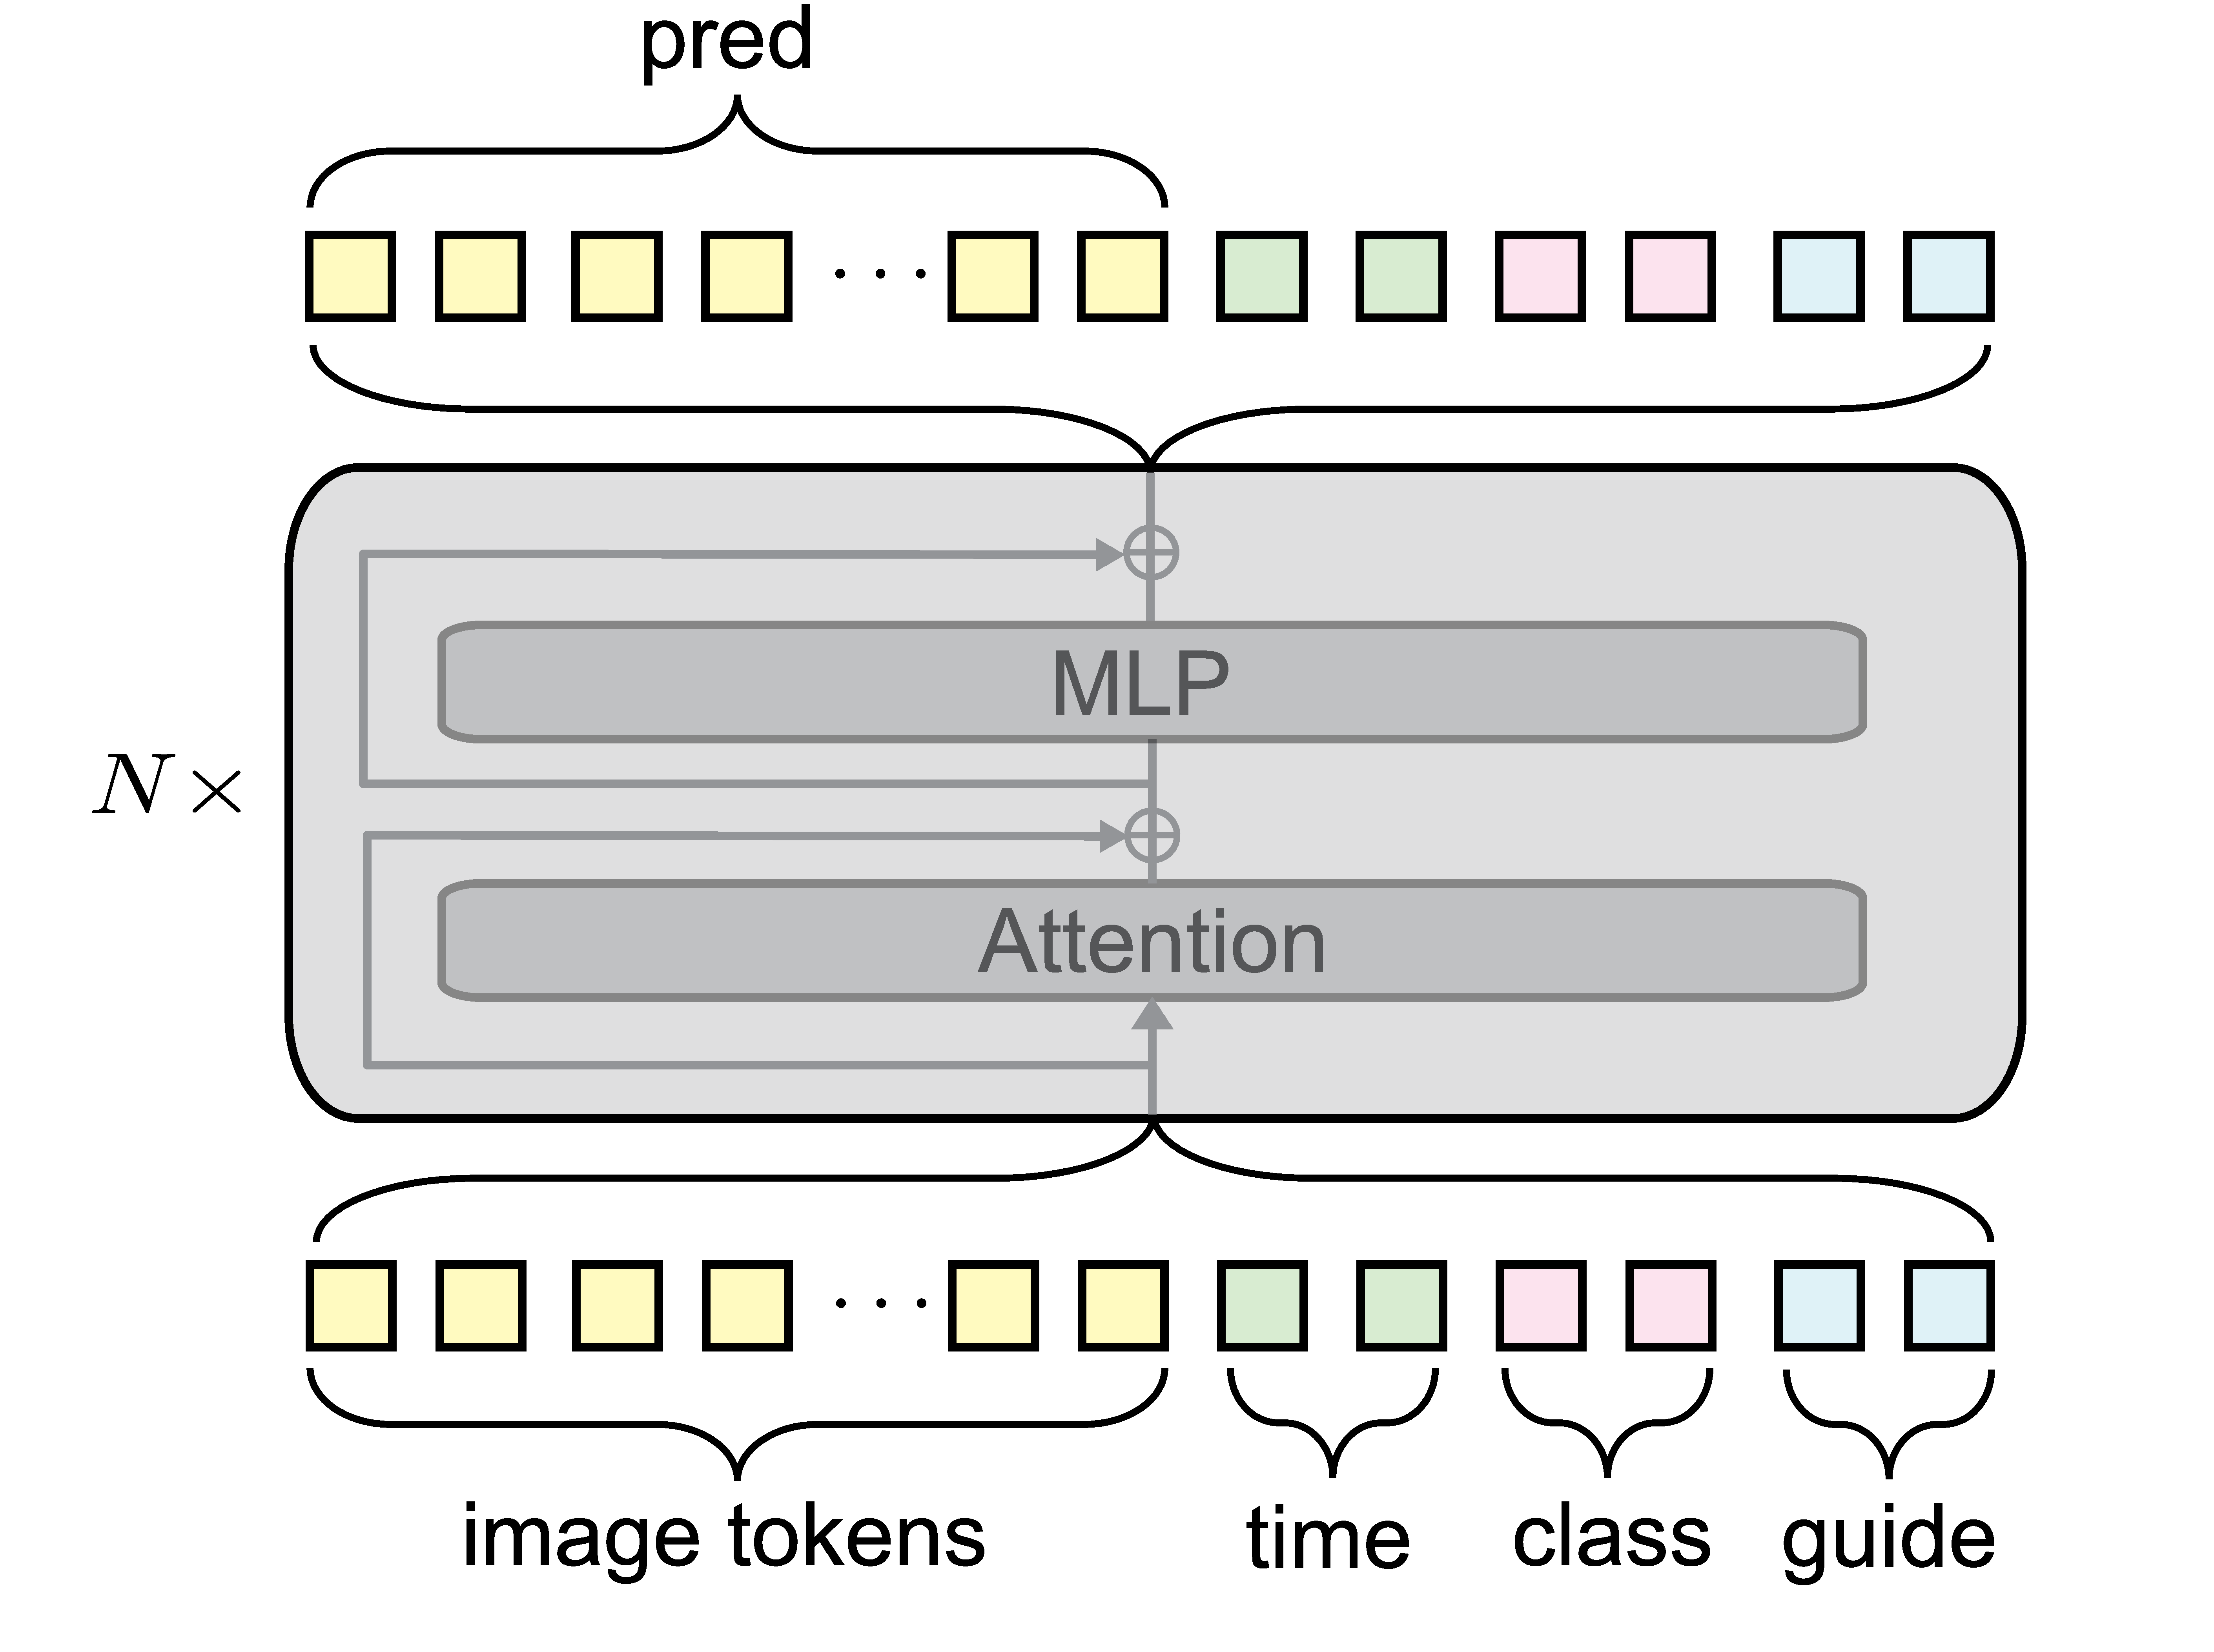
\includegraphics[width=0.8\columnwidth, angle=0,trim={0cm 0cm 0cm 0cm}, clip]{figs/arch.pdf}
    \vspace{-1em}
    \caption{\textbf{Improved in-context conditioning.}
    Each type of conditions is turned into \textit{multiple} tokens, which are concatenated with the image latent tokens along the sequence axis. It accommodates the conditions of time steps $(r,t)$, class $\mathbf{c}$, and guidance-related factors $\Omega$ (CFG scale $\omega$ and CFG intervals). Importantly, \textbf{\textit{we do not use adaLN-zero for conditioning}}, which significantly reduces the model size (number of parameters) while maintaining performance.
    }
    \label{fig:network} 
    \vspace{-1em}
\end{figure}

\subsection{Improved In-context Conditioning}
\label{sec:method-arch}

Our model has \textit{a diverse set} of conditions, including two time steps $r$ and $t$, a class label $\mathbf{c}$, and the guidance-related conditions $\Omega$. In its complete notation, the network $u_\theta$ is:
\begin{equation}
\label{eq:cond-args}
u_\theta =u_\theta\,\left(z_t \mid r,\,t,\,\mathbf{c},\,\Omega \right).
\end{equation}
Typically, the conditioning is handled by adaLN-zero \cite{dit}, which \textit{sums} all condition embeddings. When many heterogeneous conditions are present, summing their embeddings and processing by adaLN-zero may become less effective, as this single operation can be overburdened.

\paragraph{Improved MeanFlow conditioning.}
To handle these many conditions, we resort to the \textit{in-context} conditioning strategy. In-context conditioning was explored in DiT \cite{dit} but was found inferior to adaLN-zero in their setting. We find that this gap can be closed if \textit{multiple} tokens are used for each condition. In our implementation, we use 8 tokens for class, and 4 tokens for each other conditions (see appendix). 
All these learnable tokens are concatenated along the sequence axis, jointly with the tokens from images (in the latent space, same as DiT \cite{dit}). The sequence is processed by Transformer blocks (\cref{fig:network}). 
This architecture enables us to accommodate different types of conditions flexibly.


As an important by-product, our in-context conditioning enables us to completely \textit{remove} adaLN-zero, which is parameter-heavy. This yields a \textbf{1/3 reduction} in model size (\eg from 133M to 89M for our iMF-Base model) when depth and width are unchanged. This also allows us to design the larger models more flexibly.
